\documentclass[a4paper]{article}

% Encoding
\usepackage[utf8]{inputenc} % Required for inputting international characters
\usepackage[T1]{fontenc} % Output font encoding for international characters

% Bilbliography
\usepackage[style=numeric,natbib=true,giveninits=true,sorting=none]{biblatex}

% Document class "MasterDoctoralThesis" internals
\usepackage[autostyle=true]{csquotes} % Required to generate language-dependent quotes in the bibliography
\usepackage{import}
\usepackage{tocbibind}

% Images
\usepackage{graphicx} % Permet l'insertion d'image (entre autres)
\usepackage{pict2e} % Pour faire des graphiques

% Tikz and colors
\usepackage{color}
\usepackage{xcolor}
\usepackage{tikz}
	\usetikzlibrary{patterns}
	\usetikzlibrary{plotmarks}
	\usetikzlibrary{calc}
	\usetikzlibrary{shapes}
	\usetikzlibrary{arrows}
	\usetikzlibrary{fadings}

% Maths
\usepackage{amsmath} % Mathematical environnements
\usepackage{amsfonts} % Mathematical fonts
\usepackage{amssymb} % Mathematical symbols

% Tables and figures
\usepackage{array} % For tables
\usepackage{floatrow} % ??
\usepackage{subfig} % Subfigure possible
\usepackage{tabu} % Better tabular

% Misc
\usepackage[english]{babel}
\usepackage{verbatim} % Verbatim
\usepackage{bbm} % Extended blackboard bold symbols
\usepackage[colorinlistoftodos, obeyFinal]{todonotes}
\usepackage{xspace} % Trailing space for custom commands
\usepackage{hyperref}
\hypersetup{
    colorlinks,
    linkcolor={red!50!black},
    citecolor={blue!50!black},
    urlcolor={blue!80!black}
}

% Showlabel
\usepackage{showlabels}

\renewcommand{\showlabelfont}{\tiny\color{blue}}
\renewcommand{\showlabelsetlabel}[1]{\colorbox{lightgray}{\showlabelfont #1}}

% Setup
\floatsetup[figure]{style=plain,subcapbesideposition=top}
\newcommand{\bigO}[1]{\mathcal{O}\left(#1\right)} % big O notation
\newcommand{\code}[1]{\texttt{#1}} % shortcut to insert code inline
\newcommand{\EE}[1]{\cdot 10^{#1}} % power of 10
\newcommand{\missingref}{[\todo[color=blue!30, size=\tiny, caption={Missing reference}]{Missing ref}?]\xspace}
\newcommand{\myvec}[1]{\boldsymbol{\mathrm{#1}}} % bold vectors
\newcommand{\norm}[1]{\Vert #1\Vert} % norm of a vector
\newcommand{\set}[1]{\{#1\}} % set notation with curly braces
\newcommand{\total}{\text{d}} % d for total derivative


% Project specific

\newcommand{\lambdavec}{\myvec{\lambda}}
\newcommand{\uvec}{\myvec{u}}

\makeatletter

\def\@setref#1#2#3{%
  \ifx#1\relax
   \protect\G@refundefinedtrue
   \nfss@text{\reset@font\bfseries\tiny\textcolor{red}{Ref to \colorbox{lightgray}{\texttt{#3}}}}%
   \@latex@warning{Reference `#3' on page \thepage \space
             undefined}%
  \else
   \expandafter#2#1\null
  \fi}

\makeatother

\title{Degree distribution in GCC}
\author{Benoît Richard \and Guiyuan Shi}

\begin{document}

\listoftodos

\maketitle

\abstract{\todo[inline]{Write abstract}}

\section{Introduction}

Studying the fundamental properties of networks require to be able to abstract from the particular examples found in nature. This is usually done \missingref by using a random model for the network generation and averaging the properties of interest over the set of possible networks. One common model is the configuration model \missingref that allows to uniformly sample the space of all networks with a given degree distribution \missingref. However, many real examples of networks are connected, as for example the World Wide Web or railroad networks\todo{Find other examples}, but no model known to us allows to sample the space of all connected networks of a given degree distribution.

A way to still study connected networks is to only consider the Giant Connected Components (GCC) of networks generated using the configuration model \missingref. We study here how this method implies bias on the degree distribution of the GCC and propose an algorithm based on this knowledge to generate connected networks of arbitrary degree distribution.

\section{Degree distribution in GCC}

Per Bayes theorem we have for two random events $A$ and $B$
\begin{align}
	P(A | B) = \frac{P(A \cap B)}{ P(B)} = P(B | A) \frac{P(A)}{P(B)}. \label{Bayes theorem}
\end{align}
We can apply it to compute the probability $r_k$ that a vertex in the GCC has degree $k$
\begin{align}
	r_k &= P(deg(v) = k | v \in GCC)\\
	&= P(v \in GCC | deg(v) = k) \frac{P(deg(v) = k)}{P(v \in GCC)} \\
	&= (1 - P(v \notin GCC|deg(v) = k)) \frac{p_k}{S} \\
	&= \frac{p_k}{S} (1 - u^k). \label{Degree distribution in GCC},
\end{align}
where $S$ is the probability that a random node is part of the GCC, $p_k$ is the probability that a node has degree $k$ and $u$ is the probability that a node reached by following an edge of the network is not part of the GCC.\todo{More details for the last step ? Maybe a ref ?} 

In the context of the configuration model we choose the probabilities $p_k$, which determine $u$ and $S$ as
\begin{align}
	u &= \frac{\sum_{k=1}^\infty k p_k u^{k-1}}{\sum_{k=1}^\infty k p_k} \\
	S &= 1 - \sum_{k=1}^\infty p_k u^{k},
\end{align}
thus eliminating all unknown in eq. \eqref{Degree distribution in GCC}.

As seen in eq. \eqref{Degree distribution in GCC}, considering a vertex in the GCC biases the probability that it has degree $k$ by a factor $(1 - u^k)/S$. Since both $u$ and $S$ are smaller than $1$ the effect, illustrated in fig. \ref{Figure: low degree saturation}, is to lower the probability to have vertices of low degree in the GCC and to increase the probability of high degree vertices. This can intuitively understand as the fact that high degree vertices has multiple possibilities to be connected to the GCC, while low degree vertices only have few.

\begin{figure}
	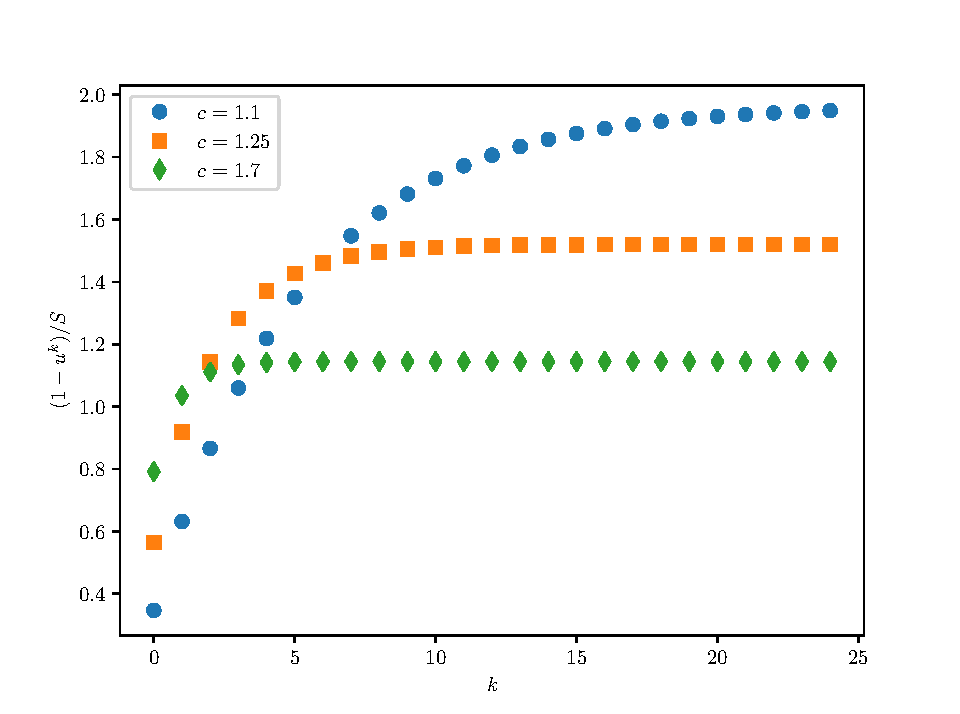
\includegraphics[width=0.8\textwidth]{drift_term.pdf}
	\caption{Bias factor $(1 - u^k)/S$ for Poisson random graph of various mean degree $c$. The closer to the critical point at $c = 1$, the larger the effect.}
	\label{Figure: low degree saturation}
\end{figure}

\section{Generating connected networks}

The knowledge of the degree distribution in the GCC can be used generate a connected component of a given degree distribution $r_k$: first we determine a degree distribution $p_k$ fulfilling eq. \eqref{Degree distribution in GCC}. Then we generate a network with degree distribution $p_k$ using the configuration model. Finally we take its GCC as our connected network. By virtue of eq. \eqref{Degree distribution in GCC} it has degree distribution $r_k$. The main problem here is to determine the $p_k$. This is hard since $u$ is a function of all $p_k$, making eq. \eqref{Degree distribution in GCC} complicated to solve. We now propose an algorithm to determine it numerically.

We first define $\tilde{p}_k = p_k/S$, giving the equations
\begin{align}
	\tilde{p}_k &= \frac{r_k}{1 - u^k} \\
	u &= \frac{\sum_{k=1}^\infty k \tilde{p}_k u^{k-1}}{\sum_{k=1}^\infty k \tilde{p}_k}\\
	p_k &= \tilde{p}_k / \sum_{k=1}^\infty \tilde{p}_k.
\end{align}
Note that the $u$ and $\tilde{p}_k$ solving this equations can be considered as being fixpoints. Iteratively inserting a guess into it should therefore make it converge towards a solution\todo{Not true in general, prove that claim ?}. Also the case $u = 1$ implies that no GCC is present and therefore does not need to be considered here.

We can not deal numerically with infinite sum, thus we choose a cutoff index $K$. We also choose a tolerance $\delta$ and a starting value $u_0$ for $u$. The algorithm then goes as follow
\begin{enumerate}
	\item Set $\tilde{p}_k := r_k$, $\forall k$ and $u_{ref} := u_0$, $u := u_0$.
	\item Compute $u_{new} := \sum_{k=1}^K k \tilde{p}_k u^{k-1} / \sum_{k=1}^K k \tilde{p}_k$.
	\item If $|u_{new} - u| > \delta$ set $u := u_{new}$ goes to 2, otherwise set $u := u_{new}$ and continue.
	\item Set $\tilde{p}_k := r_k/(1 - u^k)$, $\forall k$.
	\item If $|u_{ref} - u| > \delta$ set $u_{ref} = u$ and go back to 2, otherwise continue.
	\item Compute $p_k := \tilde{p}_k / \sum_{k=1}^\infty \tilde{p}_k$ for all $k$ and return them.
\end{enumerate}

This gives us the first $K$ probabilities $p_k$, which is sufficient to sample random numbers between $1$ and $K$ with probability $p_k$. If $K$ is chosen such that $r_k << 1$ for $k > K$, the degree distribution in the GCC closely approximate the distribution $r_k$\todo{This may not be possible for scale-free network due to fat tail, check ?}.

\begin{figure}
	\missingfigure{Plot showing residuals on the resulting $p_k$ compared to expected one.}
\end{figure}

\todo[inline]{Would be interesting to have a use case where the difference in distribution has a meaningful impact}

\section{Discussion}

\todo[inline]{Write discussion}


\end{document}